\chapter{Introduction}
\label{chapter:intro}
\setlength{\epigraphwidth}{\textwidth}
\epigraph{A picture is worth a thousand words. But how many can the machine
say?}{Our adaption of an old English proverb}

The famous English adage states "A picture is worth a thousand
words".
%%
Translated into technical terms, this is meant to convey that there is a lot the
viewer can learn/infer from a single still image and that enumerating all the
information encoded in an image can take upto even a thousand words.
%%
This is illustrated in our extensive use of images in all forms of
communication, from scientific journals to Twitter chats. 
%
Humans are very good at processing images and videos and gathering all this
encoded information, but the computers still struggle to make sense of the
simplest ones.
%
One could even say it is still easier for computers to store, parse, search and
even understand a thousand words than a single image.
%

The usage of multimedia on the internet has grown to staggering levels in the
last few yeas, due to easy access to cameras through smart phones.
%%
For example about 95 million photos are uploaded to Instagram every
day~\cite{InstStats} and about 400 hours of video is uploaded to YouTube every
minute~\cite{YouStats}.
%%
This presents both an enormous challenge and an opportunity to build smarter
computer algorithms to understand and summarize this data.
%%
Such algorithms could help us index and search this huge amount of data better.
%%
An algorithm which can learn to recognize and describe different objects and
their relationships in an image or a video would be an essential building block
of a general AI system.
%%
Hence, automatic understanding of visual media is an interesting and important
problem in many aspects of computer vision and artificial intelligence.
%

One such problem at the heart of machine understanding of visual media, is
automatic captioning of images and videos.
%%
This involves designing an algorithm which takes the image or the video as input
and generates a natural language caption describing succinctly the content of
the media.
%%
Effectively solving this problem requires the machine to be able to identify the
salient objects in the image/video, their attributes and the relationship
between these objects and also correctly recognize the scene.
%%
It also needs to be able to then use this information to generate a natural language
caption summarizing it.
%%
Since this caption generation requires both visual feature extraction and natural
language generation modules, it is also a good proxy task to measure the
progress in both these domains. 
%%

%%TODO: SHOULD THIS GO to literature review of features?
Until recently, the task of identifying even a single object in an image
reliably across diverse and large scale datasets was hard.
%%
This changed dramatically with the availability of large scale annotated data
like the ImageNet dataset~\cite{ImagenetOrig}, and  application of deep learning
techniques, specifically convolutional neural networks (CNN).
%%
For example, in the image classification task of the ImageNet Large Scale Visual
Recognition Challenge~\cite{ILSVRC15} (ILSVRC), which involves classifying
images to one of thousand object classes, the accuracy has improved from 71.8\%
to 95.06\%, surpassing the human performance on the same task. 
%%
It was also discovered that image classification networks which are trained on
the large ImageNet dataset, also generalize very well and can used as generic
image feature extraction for different tasks~\cite{yosinski2014transferable}.
%%
This has led to successful application of such deep networks to various other
tasks in computer vision including the task of image captioning.
%%

In this thesis we will examine the task of automatic image/video captioning and
discuss algorithms utilizing such tools from deep learning to solve this task.
%%
Much of the discussion presented in this thesis applies to both image and video
captioning problems.
%%
In such cases, in the interest of conciseness, we use the term "visual
captioning" to refer to both of these problems.
%%
Next, we will define the problem more precisely and list out the basic building
blocks of a visual captioning pipeline.
%%
%XXX: Talk about recent interest and mention the two stage pipeline with
%references. 

\section{Problem Statement}
\begin{figure}[th]
	\centering
	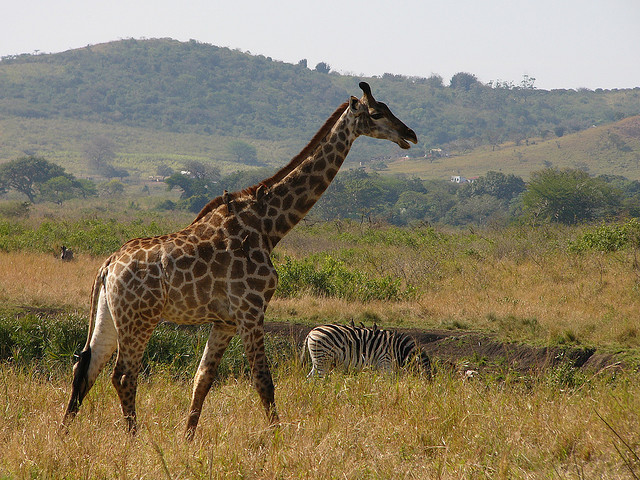
\includegraphics[width=0.8\textwidth]{./images/COCO_train2014_000000544856.jpg}\\
    \textbf{Caption:} \emph{a giraffe walking through a patch of high dried out grass.}
	\caption{A sample image--caption pair from the MS-COCO dataset.}
	\label{fig:ExampleCap}
\end{figure}

Our task is to generate a caption given an input image or video. 
%%
We are going to focus on methods to generate single sentence captions only. 
%%
Thus a caption can be precisely defined to be a sentence, $S$, which is a
sequence of words $(w_0, w_1,\cdots, w_{n-1})$ with $n$ being the length of the
sentence. 
%%
Thus we are trying to learn the distribution, $P(S|V)$, where V is the visual
input (either an image or a video). 
%%
This can be written as in eq.\ref{eq:langB1}. 

\begin{equation}
\label{eq:langB1} P(S|V) = P(w_0 w_1 \cdots w_{n-1}|V)
\end{equation}

We will take a two staged approach to model this probability distribution, as
has been popular in the image captioning literature. 
%%
In the first stage the visual input $V$ is mapped onto one or more feature
vectors $V_f$.
%%
This process is deterministic and the feature vectors extracted are of fixed
size for every input. 
%%
In this thesis, we will explore different methods for extracting feature
vectors from images and videos and analyze their performance quantitatively and
qualitatively on the automatic captioning task. 

For images, we will experiment with features extracted from CNNs trained on
ImageNet for single image classification, explicit object detector features, and
features constructed from object localization networks.
%%
In case of videos, we will explore dense trajectory features, frame-level CNN
features and 3D convolutional features. 

Next stage, is the languge model, which takes the visual feature vector $V_f$ as
input and learns a probability distibution over sentences.
%%
Since the sentences are sequence of words, they lend themselves naturally to be
modelled using sequential models like recurrent neural networks.
%%
In this thesis we will only deal with language models based on the recurrent
networks, specifically a variant called Long-Short Term Memory networks.
%%
We will implement and analyze a popular implementation proposed in
literature~\cite{Vinyals_2015_CVPR}.
%%
Then we propose some extensions to this baseline language model by adding
additional input channels, using deeper networks with residual connections,
and class based factorization of the language model. 
%%
We will also discuss several techniques to create an ensemble of language
models, exploring the problem of picking one best caption from a pool of
captions generated by each model in the ensemble.

Evaluating an image captioning system is also non-trivial, since we have to
compare the generated caption against a few different reference captions.
%%
The standard recipe followed in the literature, which we also use here, is to
use multiple automatic evaluation metrics adopted from machine translation
field. 
%%
In addition, we present human evaluation results obtained by our participation
in two automatic video captioning challenges.
%%
Concretely, we participated in the  Large Scale Movie Description
Challenge~(LSMDC) 2015 and the Microsoft Video to Text Challenge~(MSR-VTT) 2016
and we will present the results from these competition here.
%%
Our video captioning models won both the competitions as judged by human
evaluators.

We analyze the results of the experiments qualitatively and discuss strengths
and shortcomings of current solutions. 
%%
Drawing from this analysis, we discuss a few promising new directions the
research on vision and language is heading.

In summary, the main contributions of this thesis are as follows:
\begin{itemize}
  \item Discuss the basic caption generation pipeline in detail. 
  \item Propose use of alternative image and video features to improve the
          performance over the baseline model.
  \item Propose extensions to the basic language language model to improve the
          accuracy and diversity of the generated captions.
  \item Propose an effective method to ensemble multiple caption generator
          models to further improve the performance.
  \item Experiments to prove the efficacy of our proposed extensions and qualitative
          analysis of the captions generated.
  \item Identify and discuss a few promising directions of research to improve
          and extend the visual captioning systems.
       
\end{itemize}

Some content of this thesis overlaps with the three papers we have published
related to this work.
%%
Part of our experiments on image captioning has been published
in~\cite{ShettyACMMM2016Wrk}.
%%
Our video captioning solution which won the LSMDC 2015 has been published
in~\cite{shetty2015video}.
%%
Finally our video captioning system which won the MSR-VTT challenge has been
published in~\cite{ShettyACMMM2016}.
\section{Structure of the Thesis}
\label{section:structure} 
The rest of the thesis is organized as follows.
%%
In Chapter~\ref{chapter:background}, we discuss background literature related
to the building blocks of caption generation models, i.e.\@ visual feature
extraction and language modelling. 
%%
Here we will also review the several related works on visual captioning
and discuss the datasets available to train such models.
%%
We discuss the details of our baseline caption generation model and the
automatic metrics used to evaluate a captioning system in Chapter~\ref{chapter:baseline}. 
%%
Next in Chapter~\ref{chapter:VisFeatChapter} we present some extensions to
image and video features compared to the ones used in the baseline model.
%%
In Chapter~\ref{chapter:langModel}, we explore several extensions to the
baseline language model and present some ensembling techniques to combine
multiple language models.
%%
Chapter~\ref{chapter:results} contains results from several experiments to
determine the best configurations for our image and video captioning systems and
provide comparisons to few other state-of-the-art models from the literature.
%%
In Chapter~\ref{chapter:discussion}, we will identify few problem areas with our
visual captioning systems and discuss a few interesting problems to explore to
address these issues.
%%
We conclude the thesis in chapter~\ref{chapter:conclusions}.
